%!TEX program = xelatex
% 完整编译: xelatex -> bibtex -> xelatex -> xelatex
\documentclass[lang=cn,11pt,a4paper,cite=authoryear]{elegantpaper}

\title{计算机网络实验报告\\
	
\small{Computer Network Experiment Report}
}

\author{}
\institute{\href{http://imsty.cn/}{沈天宇 \\ 1851521}}

\date{\zhtoday}


% 本文档命令
\usepackage{array}
\newcommand{\ccr}[1]{\makecell{{\color{#1}\rule{1cm}{1cm}}}}
\usepackage{fancyhdr} %调用宏包

% ---基本设置---

%设定页面的页眉页脚类型,$\LaTeX$内置了四种:empty、plain、headings及myheadings,但是我们现在不用这些内置的样式。
\pagestyle{fancy}
%清除原页眉页脚样式
\fancyhf{} 
%R:页面右边;O:奇数页;\leftmark:表示"一级标题"
\fancyhead[RO]{\leftmark}
%L:页面左边;E:偶数页;\rightmark:表示"二级标题"
\fancyhead[LE]{\rightmark}
%C:页面中间
\fancyhead[CO, CE]{计算机网络实验报告}
%同上,但是不同位置放置不同信息
\fancyhead[LO, RE]{Author: 1851521 沈天宇}
% 设置页脚,页眉的位置上也可以放置页码
\fancyfoot[RO, LE]{\thepage}
\fancyfoot[LO, RE]{同济大学软件学院 \\ 计算机网络实验}
% 设置页眉页脚横线及样式
%页眉线宽,设为0可以去页眉线
\renewcommand{\headrulewidth}{0.5mm} 
%页脚线宽,设为0可以去页眉线
\renewcommand{\footrulewidth}{0.1mm} 
\begin{document}
\maketitle

\begin{abstract}
本报告为同济大学软件学院计算机网络实验报告,实验指导老师为金伟祖老师,作者为沈天宇。实验内容包括进程运行原理实验,网络端地址实验,网络线的制作和测试实验,ISO基本操作实验,UDP协议网络编程实验,TCP应用协议编程实验,端口扫描实验,物理地址解析实验,异步串联通信收发实验,主机路由实验,以太网组网实验,VLAN配置实验,虚拟无线网络实验,静态路由配置实验,蓝牙通信实验,RIP动态路由实验,OSPF动态路由实验,帧中继配置实验,以太网帧分析实验,组播实验,动态IP地址分配DHCP实验,ACL访问控制实验,邮件收发实验,IP数据包分析实验,UDP用户数据报分析实验,NAT网络地址转换实验,网络管理实验,个人文献阅读,自选型综合实验。有部分实验(比如端口扫描实验)并没有在课堂上做过但仍出现在了列表中,所以是在写报告的时候补充的。

\end{abstract}
\tableofcontents


\section{进程运行原理实验}
\subsection{实验目的}
计算机网络交互主体是计算机进程,了解进程运行的基本原理,对于理解端与进程关系十 分重要。本实验利用操作系统的进程管理软件来展示进程的生命周期。
(1)	了解进程的基本概念。
(2)	了解进程的基本运行原理,掌握基本进程管理技能。

\subsection{实验设备}
实验由一台安装Windows 10企业版操作系统的计算机担当,使用其任务管理器软件实 施进程管理实验,也可以使用其他操作系统作为操作平台。
\subsection{实验内容}
(1) 打开任务管理器。同时按"Ctrl" + "Alt" + "Delete"显示任务管理器详细信息, 显示进程运行状态信息,如图\ref{fig:renwu}所示。

\begin{figure}[htbp]
	\centering
	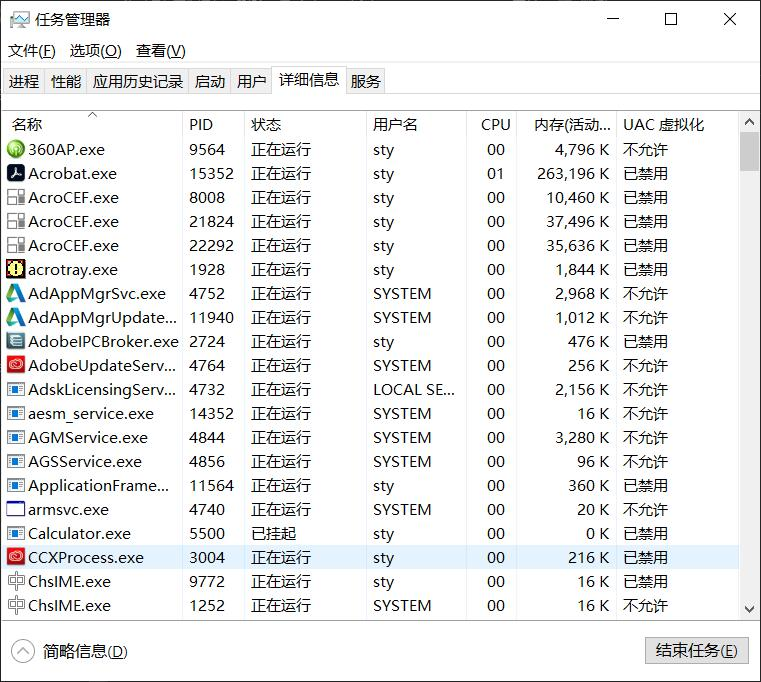
\includegraphics[width=0.7\linewidth]{screenshot001.jpg}
	\caption{进程运行状态信息}
	\label{fig:renwu}
\end{figure}
右边第一列是程序名,第二列PID列出的就是当前所有已运行程序的进程号,没有看到 命令行窗口程序(cmd)进程。

(2)	产生两个命令行窗口新进程。创建过程如图所示。

①打开两个命令行窗口。连续两次执行命令行窗口程序。
②査看命令行窗口程序的进程信息。切换到任务管理器窗口。
可以看到任务管理器窗口中新增了两行命令行程序"cmd.exe"进程信息,其进程号分别为5600和7084。

(3) 通过应用程序界面关闭进程。

1.关闭一个命令行窗口程序。
点击窗口关闭标签。

2.査看命令行窗口程序的进程信息切换到任务管理器。
可以看到进程号为5600的命令行窗口进程消失。

(4)	通过任务管理器关闭进程。
右击7084号进程-"结束进程",余下命令行窗口将被关闭,回到了原先的状态。

\subsection{实验小结}
这是一个很简单的实验,我理解了端与进程关系,了解了进程的基本概念,了解了进程的基本运行原理,掌握了基本进程管理技能。实验没有遇到困难。并且我还通过netstat -ano看到了每个进程所占用的端口号。


\section{网络端地址实验}
\subsection{实验目的}
网络端地址用于标识计算机网络进程,网络进程是计算机网络传输主体,由于语言表达上问题,容易误将计算机作为计算机网络的传输主体。明确了网络传输主体,就容易理解计算机网络各项具体功能处理的基本原理。本实验利用浏览器上网这个最为熟悉的应用,呈现网络 端地址作用。
(1)	明确计算机网络交互的主体是进程。计算机网络两台计算机之间的交互,实质上是两个进程之间的交互。
(2)	了解网络端地址构成及使用。端地址是用于标识网络上任意一台计算机上的任意一个网络进程,具有唯一性和不变性,只有通过访问网络端地址才能通过网络同该进程交互。但在日常使用应用协议时,常常忽略端口地址,自动釆用该应用协议缺省端口地址作为网络端地址。 
\subsection{实验设备}
实验环境由一台计算机来担当实验设备,计算机必须连接互联网。使用浏览器访问互联网任意一个网站,其目标网站的端地址为"www.XXX.com:80", "XXX"代表任意域名。
\subsection{实验网络拓扑}
网络端地址实验拓扑结构如图\ref{fig:screenshot001}所示。
% TODO: \usepackage{graphicx} required
\begin{figure}[htbp]
	\centering
	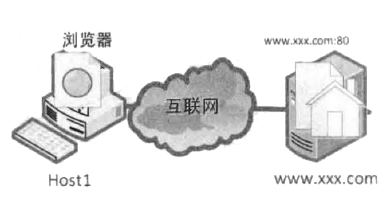
\includegraphics[width=0.7\linewidth]{image/screenshot001}
	\caption{网络端地址实验拓扑结构}
	\label{fig:screenshot001}
\end{figure}
\subsection{实验内容}
启动浏览器,通过访问同一个网址的不同端口,实验中使用了同济大学官网,实际可以是任何一个网址。

(1)	访问非80端口。地址栏中输入http://www.tongji.edu.cn:81,访问如图\ref{fig:screenshot003}所示。
% TODO: \usepackage{graphicx} required
\begin{figure}[htbp]
	\centering
	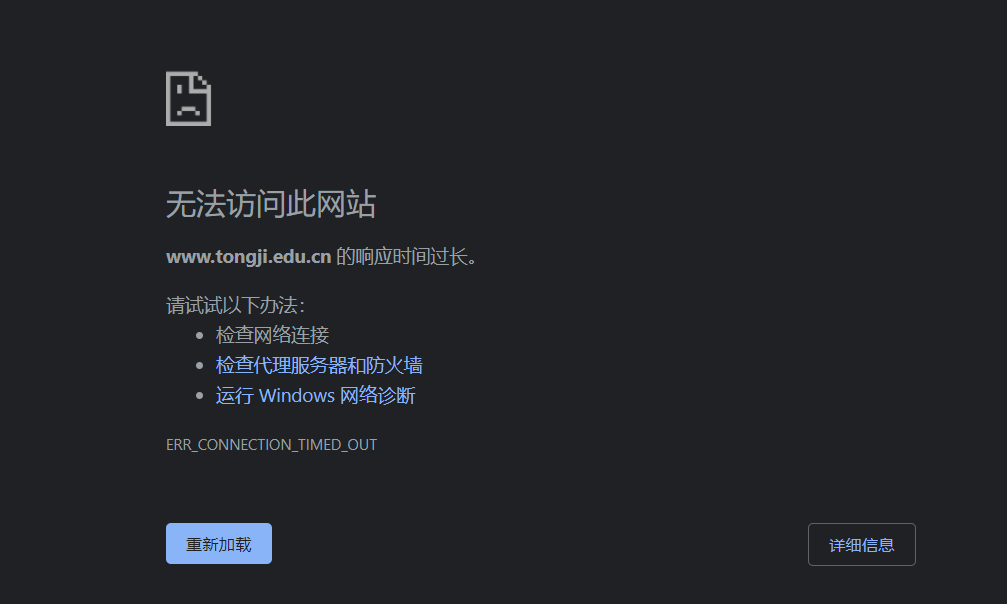
\includegraphics[width=0.7\linewidth]{image/screenshot003}
	\caption{无法访问网站}
	\label{fig:screenshot003}
\end{figure}

浏览器显示无法获得该URL地址网页,Web服务器端口地址不是81.

(2)	访问80端口,地址栏中输入"http://www.tongji.edu.cn:80",如图\ref{fig:screenshot002}所示。浏览器能正常显示网站主页内容。
% TODO: \usepackage{graphicx} required
\begin{figure}[htbp]
	\centering
	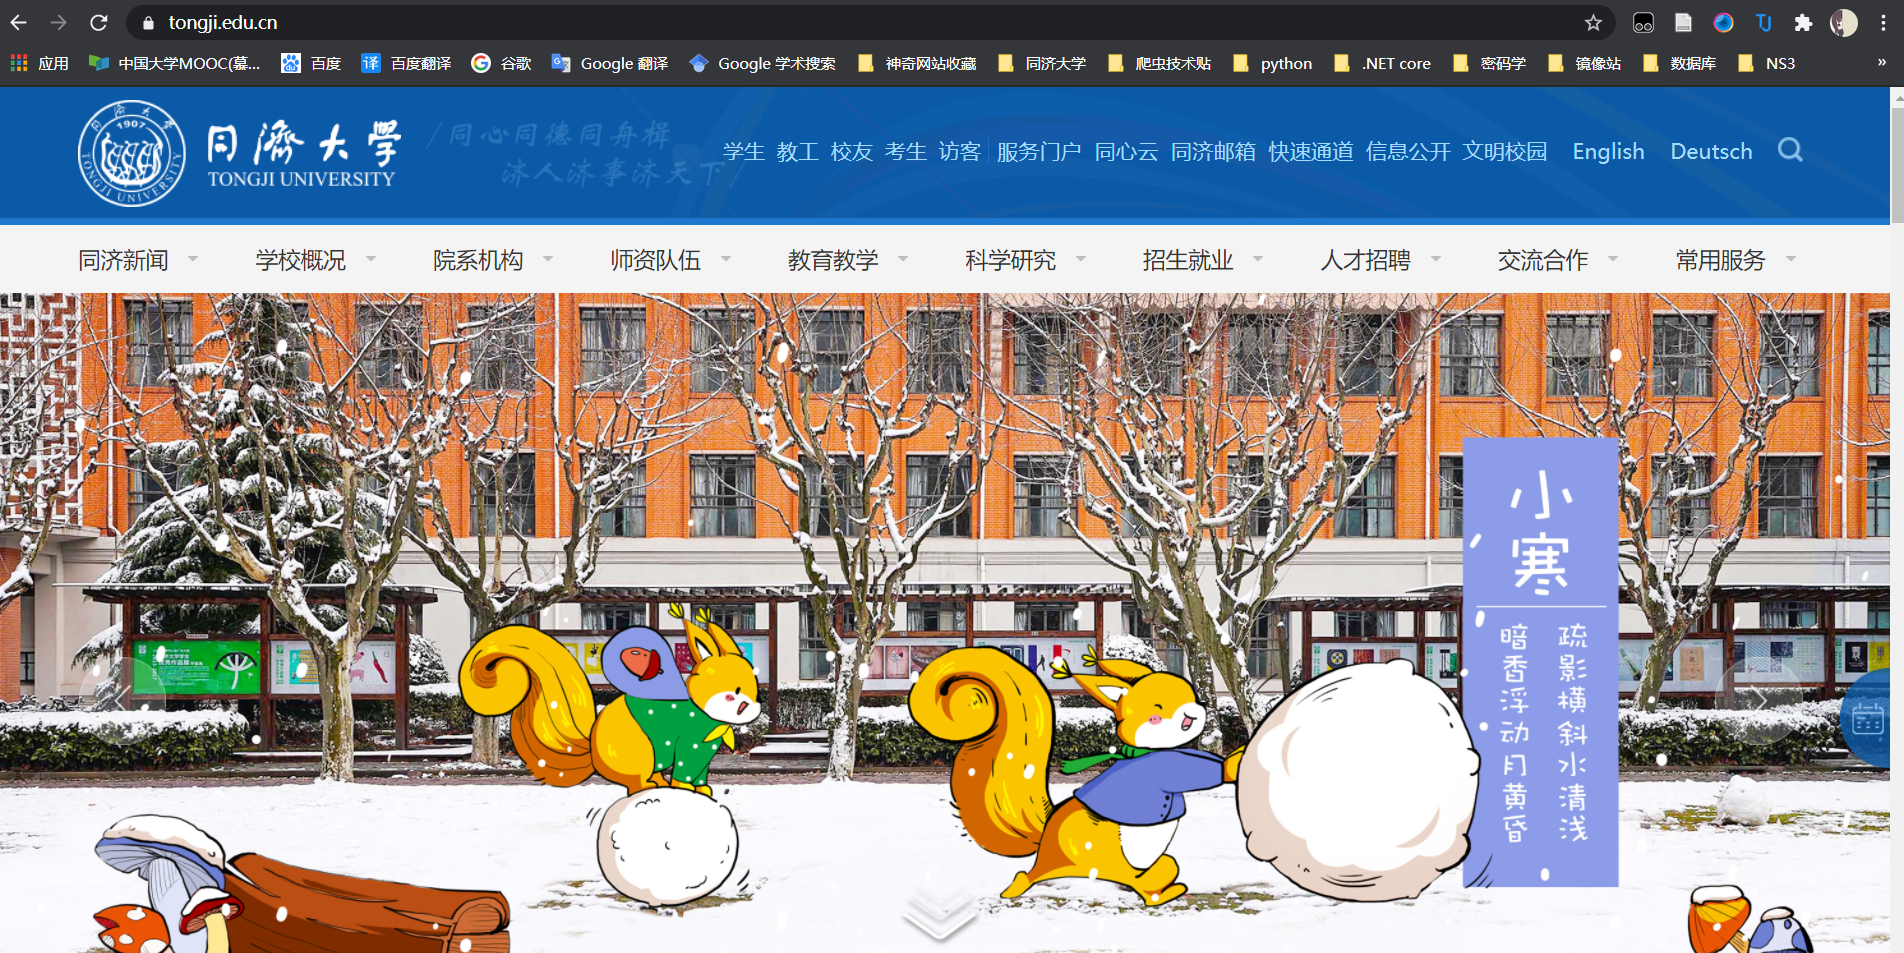
\includegraphics[width=0.7\linewidth]{image/screenshot002}
	\caption{正常访问网页}
	\label{fig:screenshot002}
\end{figure}

\subsection{实验小结}

网络端地址实验也是非常简单的实验,没有遇到任何问题。我们访问服务器的特定服务都需要指定一个特殊的端口,比如smtp协议的25端口,pop3协议的110端口,数据库使用的3306端口,https使用的443端口等等。
\section{网络线的制作和测试实验}
\subsection{实验目的}
了解以太网网络线的制作方法,深入理解物理网络的传输方式。
\subsection{实验设备}
两个TJ45水晶头,一段五类双绞线。
压线钳和网络电缆测试仪。

\subsection{实验内容}
制作一个插头,其步骤:

	1.用压线钳将网线一端的套管皮剪掉2cm。

	2.按照白橙、橙、白绿、蓝、白蓝、绿、白棕、棕线序把网线排列好。

	3.把网线摆平拉直,剪齐留下1.5cm。

	4.将水晶头有塑料弹簧片的一面向下,有金属针脚的一面向上,将线插入水晶头,并使其紧紧地顶在顶端。

	5.把水晶头插入压线钳套住水晶头用力压,使得网线和水晶头卡在一起。 

同样方法制作另一个插头

使用以太网测试工具,将网线线两端头插入网线测试仪,灯亮表示测试通过。 
\subsection{实验小结}

本次实验室我在计算机网络实验中遇到的第一个有一定难度的实验,比较考验我们的动手能力,如果没有掌握技巧,很可能在第五步"把水晶头插入压线钳套住水晶头用力压,使得网线和水晶头卡在一起"这一步失败。不过在多次尝试后,终能领略到"做网线原来如此简单"。
\section{ISO基本操作实验}
\subsection{实验目的}
1.理解实验网络物理组网原理

2.登录路由器

3.熟悉路由器操作系统ISO基本操作

\subsection{实验设备}
两台路由器,一台交换机,两台主机。

\subsection{实验网络拓扑}

% TODO: \usepackage{graphicx} required
\begin{figure}[htbp]
	\centering
	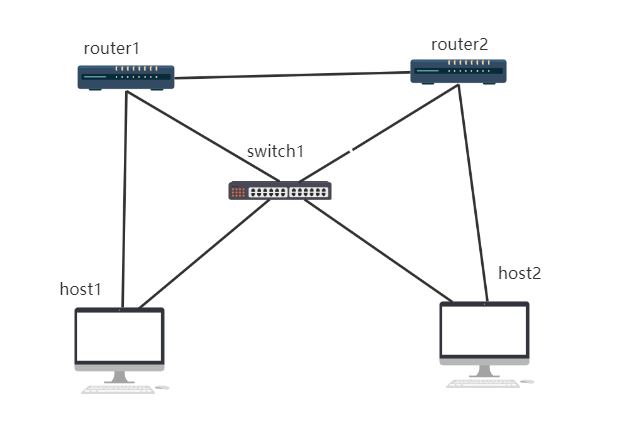
\includegraphics[width=0.7\linewidth]{image/screenshot004}
	\caption{实验网络拓扑}
	\label{fig:screenshot004}
\end{figure}

\subsection{实验内容}
\subsubsection{实验内容1}
1.观看物理连接,理解网络拓扑

2.登录路由器

--打开计算机电源

--选择系统1

--关闭防火墙

--建立HyperTerminal:开始$\rightarrow$程序$\rightarrow$附件$\rightarrow$通讯$\rightarrow$超级终端$\rightarrow$名称=router$\rightarrow$连接=com1$\rightarrow$Baut Rate=9600,8,no parity, 1 stop bit$\rightarrow$呼叫

--断开:HyperTerminal$\rightarrow$断开
\begin{table}[htbp]
\begin{tabular}{|l|l|l|l|l|}
	\hline Command Mode & Access Method & Password & Prompt Displayed & Exit Method \\
	\hline User Exec 用户 & Log in & Virtual & $>$ & Logout \\
	\hline Privileges Exec & enable & Enable Secret & $\#$ & disable \\
	\hline Global Configuration 配早 & Config t & & (config)$\#$ & Exit/ctrl+Z \\
	\hline Interface Configuration 端口配早 & Inter & & (config-if)$\#$ & Exit/ctrl+Z \\
	\hline
\end{tabular}
\caption{ISO路由器模式}
\end{table}
\subsubsection{实验内容2}
\begin{lstlisting}
ISO基本命令
1 ?
操作帮助
--寻求帮助:router01> ?
--寻求帮助:router01> sh ?
2 show
--寻求帮助:router01> sh ?
--查看系统配置:router01> sh version
--查看路由表:router01>sh ip route
--寻求帮助:router01> sh ?
--寻求帮助:router01> sh in ?
--寻求帮助:router01> sh int g ?
--查看以太网口配置:router01> sh int gt 0/0
--寻求帮助:router01> sh int ser ?
--查看串口配置:router01> sh int serial 0/0
--查看路由表配置信息:router01> sh running-config  #权限不够
3 enable
--进入特权模式:router01>en(able) ,Enable Secret Password=cisco
--查看路由表配置信息:router01# sh running-config 
--寻求帮助:router01# sh int g ?
--查看以太网口配置:router01# sh in g 0/0
--寻求帮助:router01# sh int ser ?
--查看串口配置:router01# sh int serial 0/0
4 config
--进入配置模式:router01#config t
--寻求帮助:router01(config)# ?
5 interface
--寻求帮助:router01# inter fast ?
--进入以太口:router01(config)#int g 0/0
--修改IP地址: router01(config-if)#ip address 192.168.x.2
6 end
--退到特权模式:router01(config-if)#end(ctrl+z), exit
--查看以太网口配置:router01# sh int g 0/0
7 ping 
--连通测试命令: router01# ping 192.168.x.254
8 shut
关闭端口
--进入配置模式:router01#config t
--进入以太口:router01(config)#int g 0/0
--关闭端口功能:router01(config-if)#no shut
--退到特权模式:router01(config-if)#end(ctrl+z), exit
--查看以太网口配置:router01# sh int g 0/0
9 no
反命令
--进入配置模式:router01#config t
--进入以太口:router01(config)#int g 0/0
--打开端口功能:router01(config-if)#no shut
--退到特权模式:router01(config-if)#end(ctrl+z), exit
--查看以太网口配置:router01# sh int gt 0/0
--进入以太口:router01(config)#int g 0/0
--删除IP地址: router01(config-if)#no ip address <ipaddress><subnet mask>

\end{lstlisting}
\subsection{实验小结}
本次实验是ISO路由器基本操作试验,是后面所有实验的基础,因为后面的每次实验都需要通过命令行来操作路由器和交换机。实验内容非常简单,只需要跟着教程做就可以做出来了,本次实验了解了很多ISO操作系统的常用命令,为后面的实验打好了基础。

\section{UDP协议网络编程实验}
\subsection{实验目的}
UDP协议应用面没有TCP协议广,但影响也很大,如微信和QQ等都是典型的UDP应用。UDP网络编程原理基本相同。本实验是使用Socket来编写一个基于UDP简易通信程序,进行即时通信。

(1)	理解客户机/服务器模型,了解端口在网络传输中的作用。

(2)	了解无连接通信方式及编程方式。

(3)	了解掌握基于Socket的UDP应用编程的基本步骤。 

\subsection{实验设备}
一台安装了java的电脑,老师使用的IDE是Eclipse,我使用的是IDEA.
\subsection{实验内容}
运行Eclipse开发平台,并选择已创建Socket项目。

(1)	创建Java包"edu.tongji.networklab.udp"

右击项目 "MSocket/Java Resources/srcw"

"New"->"Package"

输入包名"Name=edu.tongji.networklab.udp"->"Finish"。创建该包用于存放 UDP 实验类。

(2)	开发UdpClient类。

	1.创建 UdpClient类。在包"edu.tongji.networklab.udp"下,创建 UDPClient类。 

右击"src/edu.tongji.networklab.udp"->"New"->"Class".

Name=UdpClient,选择"public static void main(String[ ] arg) "—>"Finish".

	2.输入实验代码。用附录2中UdpCIient源代码完全覆盖初始代码

	3.保存。保存包含着对Java编译,键入"Ctrl+S"或菜单"File"—>"Save"。

(3)	开发UdpServer类

	1.创建 UdpServer 类;类似 UdpCIient,在"edu.tongji.networklab.udp"下,创建 UDPServer类。 

右击"src/edu.tongji.networklab.udp"->"New"->"Class"->"Name=UdpServer",选择"public static void main(String[ ] args)"—>"Finish"

	2.代码开发。输入实验源代码,用附录2中UdpServer源代码完全覆盖初始代码。

	3.保存。保存包含着对Java编译,键入"Ctrl + S"或菜单"File"->"Save"。

(4)代码运行测试。

	1.运行UdpServerC

右击UdpServer—"Run as"->"Java Application"。

	2.运行 UdpClient 发送。同上,右击"UdpClient"->"Run as"->"Java Application"。

点击"连接",然后在发送区输入"hello"->"发送"。

	3.接收文本。
UdpClient的接收区显示"hello";左下角是UdpServer控制台,显示UdpServer收到的客户端请求数据"hello",实验成功。

下面是本次实验的截图。

% TODO: \usepackage{graphicx} required
\begin{figure}[htbp]
	\centering
	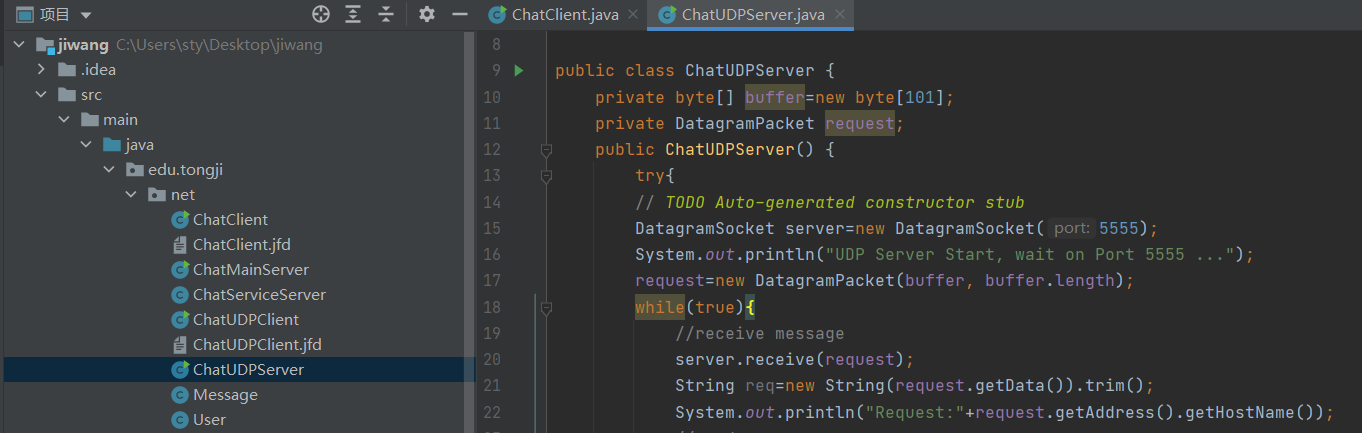
\includegraphics[width=0.9\linewidth]{image/screenshot006}
	\caption{部分代码截图}
	\label{fig:screenshot006}
\end{figure}


% TODO: \usepackage{graphicx} required
\begin{figure}[htbp]
	\centering
	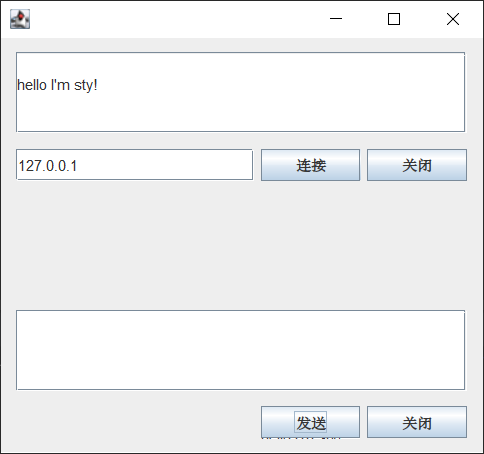
\includegraphics[width=0.7\linewidth]{image/screenshot005}
	\caption{实验截图}
	\label{fig:screenshot005}
\end{figure}


\subsection{实验小结}
(这个实验上课好像没有讲)实验代码金老师已经帮我们写好了,所以我们很快做完了实验,但是关键是要领会试验运行的原理,而不是只关注实验运行的结果。

\section{TCP应用协议编程实验}
\subsection{实验目的}
TCP是使用最为广泛的传输层协议,绝大多数的网络应用服务器都使用TCP协议以保证数据传输可靠,但工程上服务器还需要具有并发能力,允许多个客户并发访问。本实验是使用Socket来编写一个基于TCP简易通信程序,且具有并发能力。
(1)	了解基于TCP网络应用服务器的基本编程架构。
(2)	了解面向连接和无连接的区别,了解TCP编程基本步骤。
(3)	了解并发服务原理及编程方式。

\subsection{实验设备}
一台安装了java的电脑,老师使用的IDE是Eclipse,我使用的是IDEA.

\subsection{实验内容}
创建实验项目目录的过程和上一个实验相似,这里不再赘述。关键点如下:

在Java项目Socket下,开发服务器程序和客户机程序。

(1)	开发服务器程序,创建并实现MainServer类和ServiceServer类,将附录3的MainServer类和ServiceServer类全部源代码复制进去。

(2)	开发客户机程序TCPClient类,为方便实验,TCPClient包含图形化界面,代码较长,将附录3的TCPClient全部源代码复制进去。

(3)	测试交互。先运行MainServer,后运行TCPClient,将连续创建两个TCPClient进程,并同时访问服务器,然后在TCPClient界面中输入字符串,测试并发通信服务。

下面是本次实验我的截图,如图\ref{fig:screenshot008} 图\ref{fig:screenshot007}:

% TODO: \usepackage{graphicx} required
\begin{figure}[htbp]
	\centering
	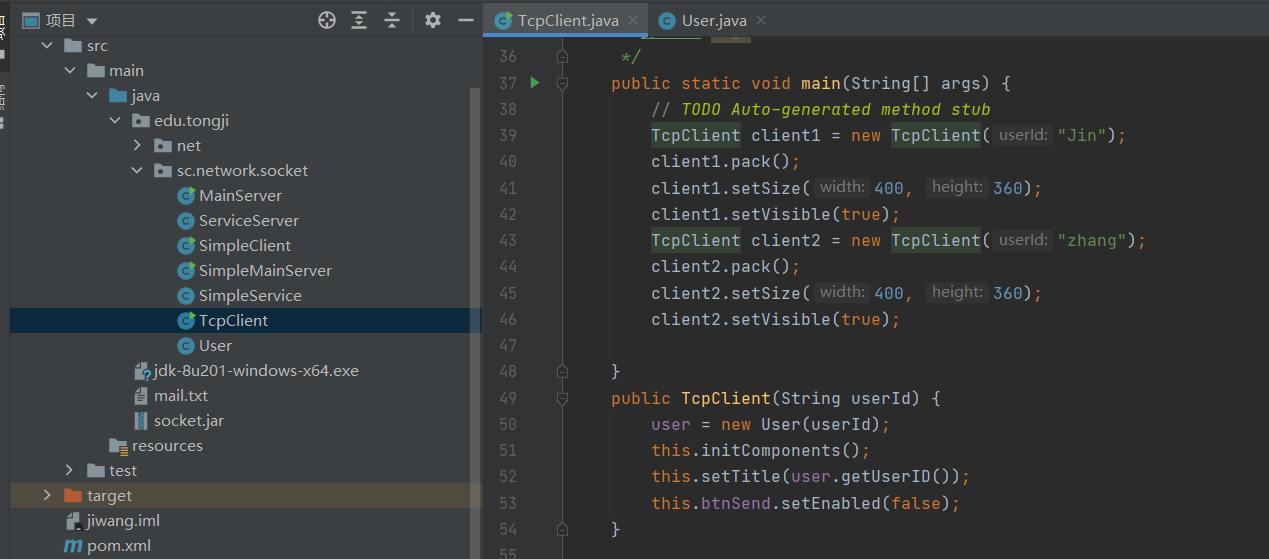
\includegraphics[width=0.8\linewidth]{image/screenshot008}
	\caption{部分代码截图}
	\label{fig:screenshot008}
\end{figure}


% TODO: \usepackage{graphicx} required
\begin{figure}[htbp]
	\centering
	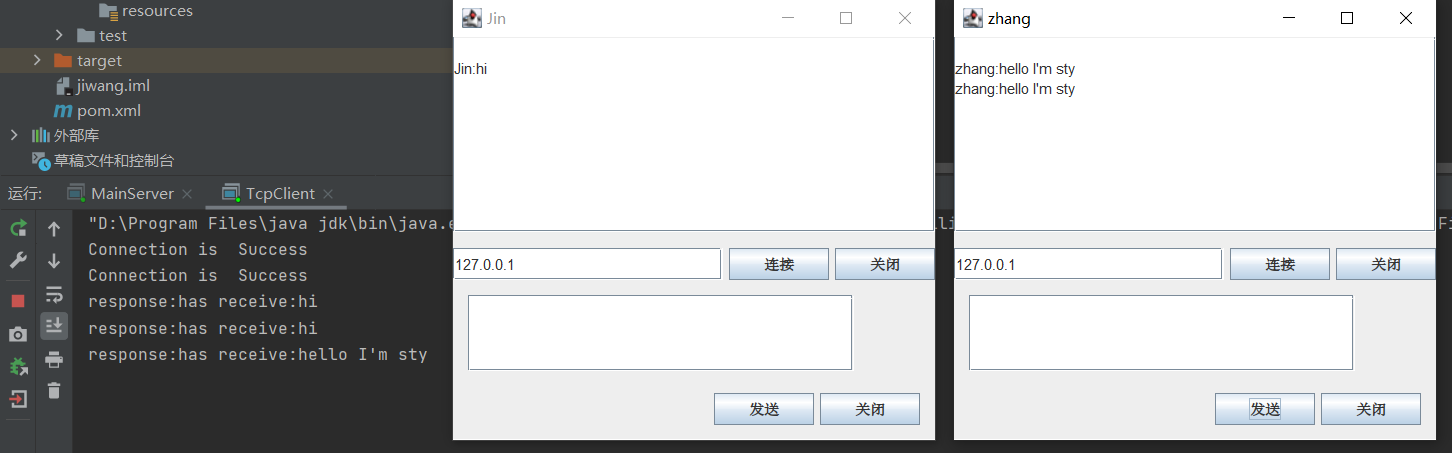
\includegraphics[width=0.8\linewidth]{image/screenshot007}
	\caption{实验截图}
	\label{fig:screenshot007}
\end{figure}


\subsection{实验小结}
这个实验和上个实验很像,TCP和UDP都是传输层协议,但具体的细节有很多很多的不同。实验代码金老师已经帮我们写好了,所以我们很快做完了实验,但是关键是要领会试验运行的原理,而不是只关注实验运行的结果。
\section{端口扫描实验}
\subsection{实验目的}
端口扫描是应对主机入侵而釆取的基本防范措施,掌握端口管理的基本技能是应对网络攻击的必备技能。本实验将使用开源的专业端口扫描软件工具nmap,对子网内的主机进行端口扫描。
(1)	了解端口开放含义。
(2)	了解安全漏洞含义。
(3)	了解掌握网络漏洞扫描工具的使用。
(4)	使用服务管理对端口进行管理。

\subsection{实验设备}

主机需要安装nmap软件。两台计算机和一台交换机担当实验设备,使用两根以太网络线,将两台计算机网卡和交换机连接起来,构成一个子网。主机Hostl作为端口扫描操作平台,另一台主机Host2作为扫描的目标平台,可以是任何一种操作系统,目标主机安装 Windows。在操作平台上使用端口扫描工具软件对目标主机进行扫描。实验使用Windows版本nmap作为端口扫描工具软件,nmap是一款开源的软件,需要下载安装。

\subsection{实验网络拓扑}

% TODO: \usepackage{graphicx} required
\begin{figure}[htbp]
	\centering
	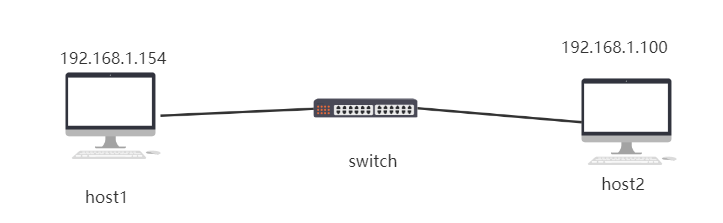
\includegraphics[width=0.7\linewidth]{image/screenshot009}
	\caption{端口扫描网络拓扑}
	\label{fig:screenshot009}
\end{figure}

\subsection{实验内容}

\subsubsection{实验一:远程子网扫描实验}

(1)	配置主机Hostl和Host2地址,主机网卡IP地址设置如下: 

Hostl:IP 地址= 192. 168.1.254,子网掩码=255.255.255.0,网关= 192.168.1.1

Host2:IP 地址= 192. 168. 1.100,子网掩码= 255.255.255.0,网关= 192.168.1.1

(2)	使用nmap扫描软件远程扫描指定子网。对192.168.1.0/24子网进行扫描。

1.Hostl 上启动 nmap。

左击“开始”->“所有程序”->“Nmap”->“Nmap-Zenmap GUI”。

2.扫描192. 168. 1.0/24子网。

输入“目标= 192. 168. 1. * ”,配置=Intense scan->“扫描”,注意扫描要持续一段时间,请保持耐心,在左边会依次列出被扫描的主机IP地址。

3.査看目标主机的端口开放状况。

选择主机192. 168. 1.100,点击“端口/主机”发现了10个开放的端口。

\subsubsection{实验二:端口关闭实验}

如果发现某些端口不用开放,就可以关闭这些端口。实验将关闭目标主机上VM认证服务端口。

(1)进入服务,关闭目标主机上VM认证服务。Host2,右击“开始”->“系统”->“其他管理工具”->“管理工具”->“服务"。

右击 VMware Anthorization Service->“停止”。

(2)重新扫描192.168.1. 100核实。由于nmap是个优秀的软件,所以只要实验网络拓扑没有断开,实验很容易就取得了成功。

实验结果如下图:

% TODO: \usepackage{graphicx} required
\begin{figure}[htbp]
	\centering
	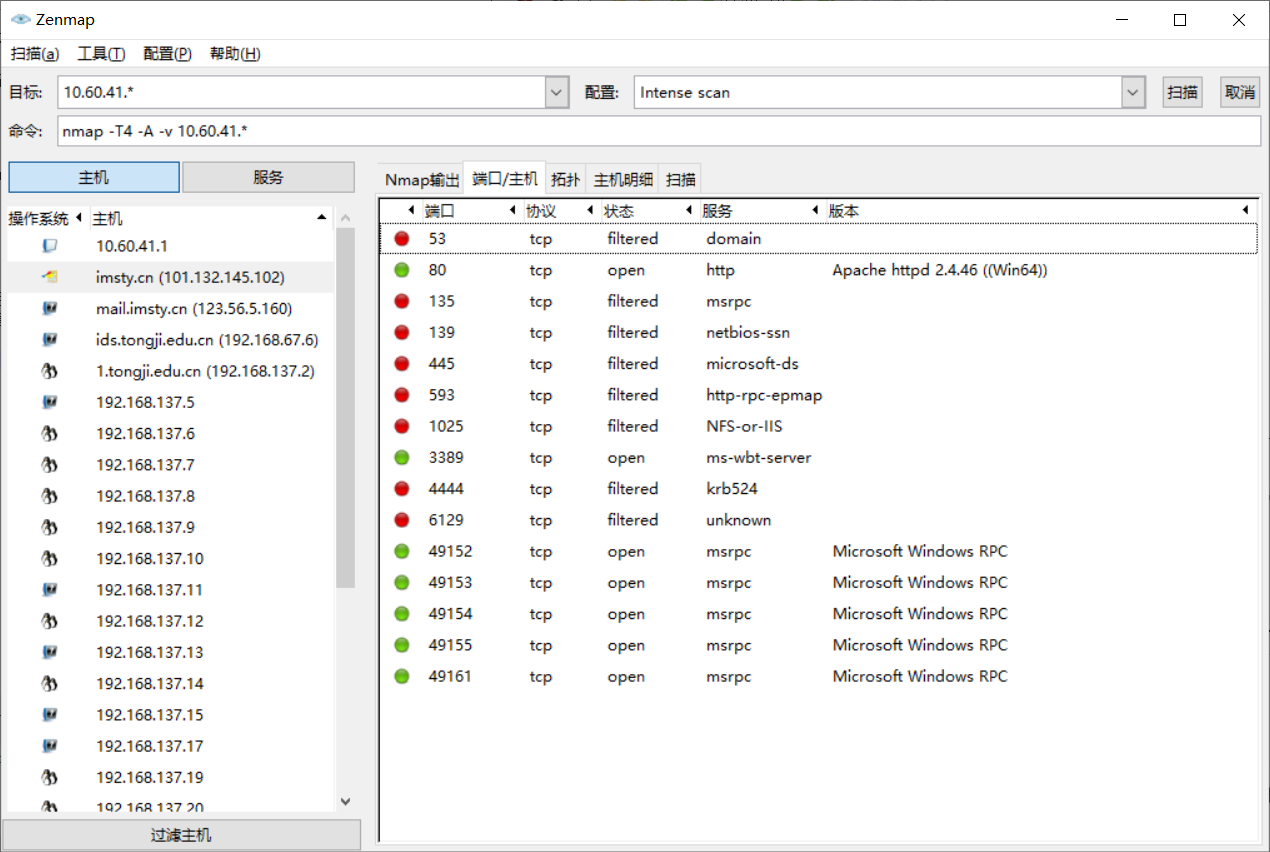
\includegraphics[width=0.7\linewidth]{image/screenshot010}
	\caption{端口扫描}
	\label{fig:screenshot010}
\end{figure}


\subsection{实验小结}
这个实验我记得其实上课金老师没带我们做,是我课后根据实验列表自己补上的。实验让我对端口扫描有了一个从感性到理性的认识,开放的网络端口确实比较容易给黑客以可乘之机,这让我想起了臭名昭著的勒索病毒WannaCry,它就是利用了Windows操作系统445端口存在的漏洞。
\section{物理地址解析实验}
\subsection{实验目的}
IP网络不具有实际通信能力,需要将IP数据包封装在物理帧中进行传输,封装前需要对下一跳IP地址进行物理地址解析。物理地址解析是理解IP封装的关键知识点,但物理地址解析行为非常隐蔽,难以察觉。实验利用ARP协议的缓存机制来间接证明物理地址解析行为的发生:
(1)	理解IP网络和物理网络之间的功能关系。
(2)	了解ARP地址解析原理。
(3)	掌握ARPT具软件使用。

\subsection{实验设备}

两台计算机和一台交换机担当实验设备,使用两根以太网络线,将两台计算机网卡都用网 线直接连接交换机。主机Hostl作为地址解析源节点,另一台主机Host2作为地址解析目标节点。使用Windows操作系统自带的ARP工具软件作为实验工具。

\subsection{实验网络拓扑}
% TODO: \usepackage{graphicx} required
\begin{figure}[htbp]
	\centering
	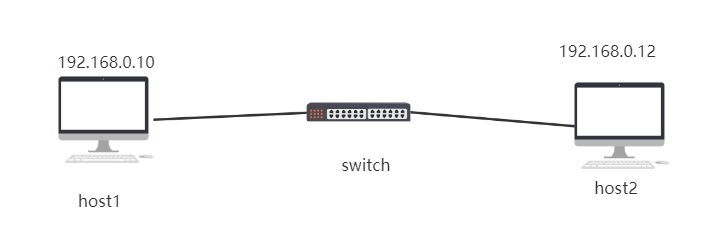
\includegraphics[width=0.7\linewidth]{image/screenshot011}
	\caption{实验网络拓扑}
	\label{fig:screenshot011}
\end{figure}


\subsection{实验内容}

按照实验环境要求,完成实验拓扑结构连接,并打开相关设备电源。

(1)	为Host1和Host2设置IP地址。主机网卡IP地址设置如下:

Host1:IP 地址= 192.168.0.12,子网掩码= 255. 255. 255.0,网关空缺

Host2:IP 地址= 192.168.0.10,子网掩码= 255. 255. 255.0,网关空缺

(2)	Host2触发对Hostl的地址解析。解析如图4-10和图4-11所示。

1.Host2清除ARP缓存表。Host2以管理员身份打开命令行窗口,清除ARP缓存表,以消除有可能存在192. 168. 0.12地址解析条目。

输入:arp-d,清空地址解析缓冲区,以便消除可能已产生的地址解析;

arp -a,显示当前地址解析缓冲区内容,没有出现192. 168.0. 12条目。

2.Host2触发对Host1地址解析,并获得其地址解析缓存。Host2发出ping连通测试命令。

输入“ping 192. 168.0. 12”,测试连通Hostl,触发对192. 168.0. 12的地址解析。

arp-a,显示当前地址解析缓存表内容,岀现了192. 168.0. 12条目,说明在发出连通测试IP数据包前,对192. 168. 0. 12节点的物理地址进行了解析,其解析物理地址是78-36-cc-ee-ab-39。

(3)	核实解析物理地址。Host1打开命令行窗口,核实物理地址。

输入“ipconfig /all”,列出IP地址和物理网卡地址,IP地址是192. 168. 0. 12,物理地址是78-36-cc-ee-ab-39,同Host2解析得到的物理地址完全一致。

实验结果如图\ref{fig:arp} 和图\ref{fig:screenshot012}所示,注意图中红框。

\begin{figure}[htbp]
	\centering
	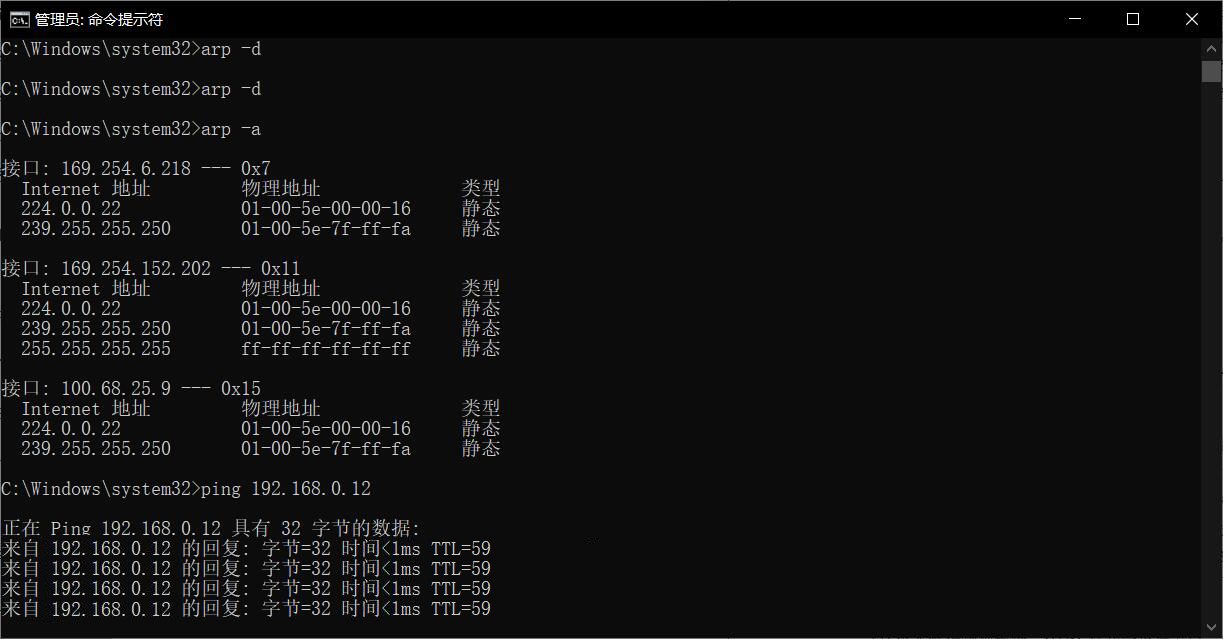
\includegraphics[width=0.7\linewidth]{arp.jpg}
	\caption{物理地址解析实验}
	\label{fig:arp}
\end{figure}


\begin{figure}[htbp]
	\centering
	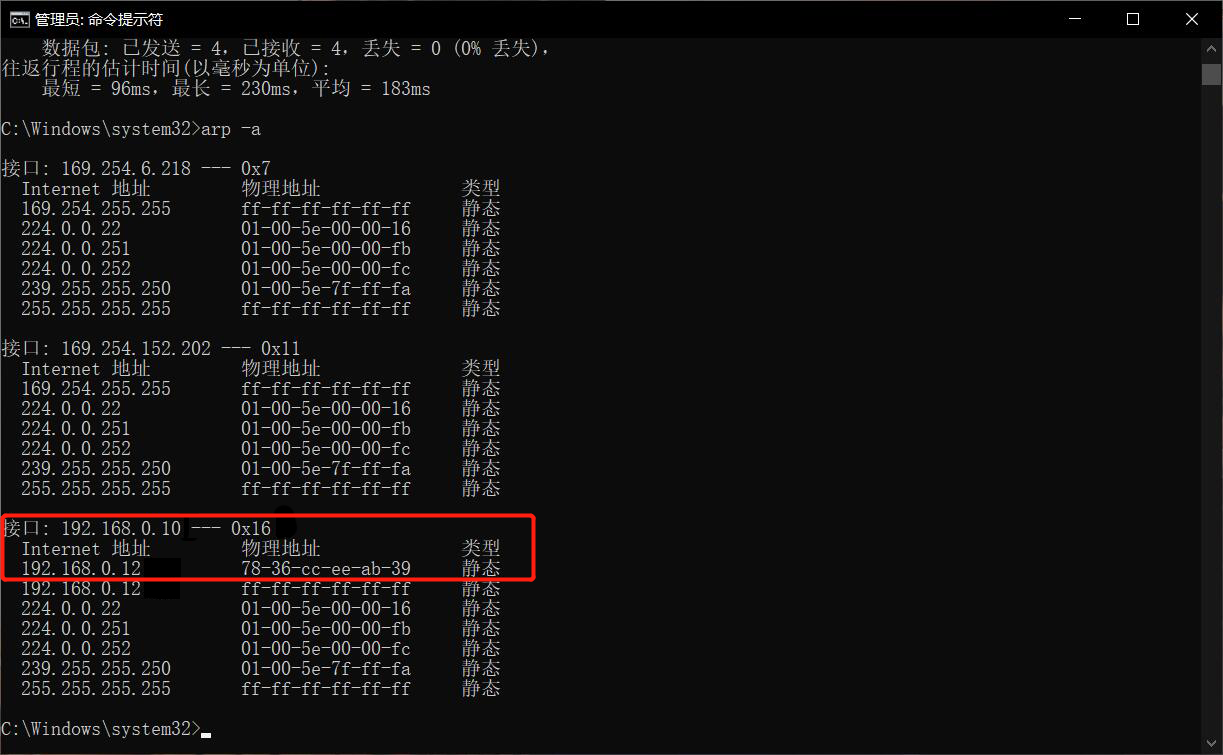
\includegraphics[width=0.7\linewidth]{image/screenshot012}
	\caption{物理地址解析实验图2}
	\label{fig:screenshot012}
\end{figure}


\subsection{实验小结}
物理地址解析实验也是非常重要的实验,实验本身没什么难度,关键在于理解。物理地址解析是通过广播ARP消息来完成的,相当于向局域网里所有主机发出一个问题:“谁拥有IP地址xxx.xxx.xxx.xxx?”然后拥有这个IP地址的主机就会回应。


\section{异步串联通信收发实验}
\subsection{实验目的}
数据通信是物理层的核心功能,其基本原理属于通信学范畴。实验利用计算机的COM口进行两台计算机间的字符收发,展示通信基本原理,加深了解物理层作用。
(1)	理解异步串行通信基本原理。
(2)	熟悉掌握RS-232通信标准以及RS-232帧格式。
(3)	了解波特率等主要通信参数的作用和使用。

\subsection{实验设备}

1. 实验环境主要由两台带COM口的计算机,1根串行交叉线组成;
2. 将单根串行交叉线中间层组成。将单根串行交叉线将两个计算机的COM串口对接起来;
3. 两台计算机超级终端将作为路由器管理的操作平台。

\subsection{实验网络拓扑}

% TODO: \usepackage{graphicx} required
\begin{figure}[htbp]
	\centering
	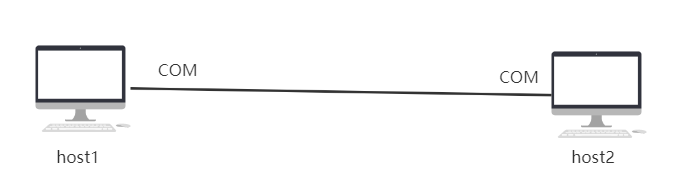
\includegraphics[width=0.7\linewidth]{image/screenshot013}
	\caption{异步串行通信试验网络拓扑}
	\label{fig:screenshot013}
\end{figure}

实验环境主要由两台带COM口的计算机,一根串行交叉线组成。将单根串行交叉线将两个计算机的COM串口对接起来;两台计算机超级终端将作为路由器管理的操作平台。

\subsection{实验内容}
\subsection{实验小结}
\section{主机路由实验}
\subsection{实验目的}
\subsection{实验设备}
\subsection{实验网络拓扑}
\subsection{实验内容}
\subsection{实验小结}
\section{以太网组网实验}
\subsection{实验目的}
\subsection{实验设备}
\subsection{实验网络拓扑}
\subsection{实验内容}
\subsection{实验小结}
\section{VLAN配置实验}
\subsection{实验目的}
\subsection{实验设备}
\subsection{实验网络拓扑}
\subsection{实验内容}
\subsection{实验小结}
\section{虚拟无线网络实验}
\subsection{实验目的}
\subsection{实验设备}
\subsection{实验网络拓扑}
\subsection{实验内容}
\subsection{实验小结}
\section{静态路由配置实验}
\subsection{实验目的}
\subsection{实验设备}
\subsection{实验网络拓扑}
\subsection{实验内容}
\subsection{实验小结}
\section{RIP动态路由实验}
\subsection{实验目的}
\subsection{实验设备}
\subsection{实验网络拓扑}
\subsection{实验内容}
\subsection{实验小结}
\section{OSPF动态路由实验}
\subsection{实验目的}
\subsection{实验设备}
\subsection{实验网络拓扑}
\subsection{实验内容}
\subsection{实验小结}
\section{帧中继配置实验}
\subsection{实验目的}
\subsection{实验设备}
\subsection{实验网络拓扑}
\subsection{实验内容}
\subsection{实验小结}
\section{组播实验}
\subsection{实验目的}
\subsection{实验设备}
\subsection{实验网络拓扑}
\subsection{实验内容}
\subsection{实验小结}
\section{动态IP地址分配DHCP实验}
\subsection{实验目的}
\subsection{实验设备}
\subsection{实验网络拓扑}
\subsection{实验内容}
\subsection{实验小结}
\section{ACL访问控制实验}
\subsection{实验目的}
\subsection{实验设备}
\subsection{实验网络拓扑}
\subsection{实验内容}
\subsection{实验小结}
\section{邮件收发实验}
\subsection{实验目的}
\subsection{实验设备}
\subsection{实验网络拓扑}
\subsection{实验内容}
\subsection{实验小结}
\section{ARP消息分析实验}
\subsection{实验目的}
\subsection{实验设备}
\subsection{实验网络拓扑}
\subsection{实验内容}
\subsection{实验小结}
\section{IP数据包分析实验}
\subsection{实验目的}
\subsection{实验设备}
\subsection{实验网络拓扑}
\subsection{实验内容}
\subsection{实验小结}
\section{UDP用户数据报分析实验}
\subsection{实验目的}
\subsection{实验设备}
\subsection{实验网络拓扑}
\subsection{实验内容}
\subsection{实验小结}
\section{NAT网络地址转换实验}
\subsection{实验目的}
\subsection{实验设备}
\subsection{实验网络拓扑}
\subsection{实验内容}
\subsection{实验小结}
\section{个人文献阅读}
\section{自选型综合实验}
\subsection{实验目的}
\subsection{实验设备}
\subsection{实验网络拓扑}
\subsection{实验内容}
\subsection{实验小结}

\subsection{模板介绍}

此模板基于 \LaTeX{} 的标准文类 article 设计,所以 article 文类的选项也能传递给本模板,比如 \lstinline{a4paper, 11pt} 等等。本模板支持 \hologo{pdfLaTeX} 和 \hologo{XeLaTeX} 编译。

\begin{lstlisting}
\documentclass[a4paper,11pt]{elegantpaper}
\end{lstlisting}

\textbf{注意}:Elegant\LaTeX{} 系列模板已经全部上传至 \href{https://www.overleaf.com/latex/templates/elegantpaper-template/yzghrqjhmmmr}{Overleaf} 上,用户可以在线使用。另外,为了方便国内用户,模板也已经传至\href{https://gitee.com/ElegantLaTeX/ElegantPaper}{码云}。


\subsection{全局选项}
此模板定义了一个语言选项 \lstinline{lang},可以选择英文模式 \lstinline{lang=en}(默认)或者中文模式 \lstinline{lang=cn}。当选择中文模式时,图表的标题引导词以及参考文献,定理引导词等信息会变成中文。你可以通过下面两种方式来选择语言模式:
\begin{lstlisting}
\documentclass[lang=cn]{elegantpaper} % or
\documentclass{cn}{elegantpaper} 
\end{lstlisting}

\textbf{注意:} 英文模式下,由于没有添加中文宏包,无法输入中文。如果需要输入中文,可以通过在导言区引入中文宏包 \lstinline{ctex} 或者加入 \lstinline{xeCJK} 宏包后自行设置字体。 
\begin{lstlisting}
\usepackage[UTF8,scheme=plain]{ctex}
\end{lstlisting}

\subsection{数学字体选项}

本模板定义了一个数学字体选项(\lstinline{math}),可选项有三个:
\begin{enumerate}
  \item \lstinline{math=cm}(默认),使用 \LaTeX{} 默认数学字体(推荐,无需声明);
  \item \lstinline{math=newtx},使用 \lstinline{newtxmath} 设置数学字体(潜在问题比较多)。
  \item \lstinline{math=mtpro2},使用 \lstinline{mtpro2} 宏包设置数学字体,要求用户已经成功安装此宏包。
\end{enumerate}

\subsection{中文字体选项}
模板提供中文字体选项 \lstinline{chinesefont},可选项有
\begin{enumerate}
\item \lstinline{ctexfont}:默认选项,使用 \lstinline{ctex} 宏包根据系统自行选择字体,可能存在字体缺失的问题,更多内容参考 \lstinline{ctex} 宏包\href{https://ctan.org/pkg/ctex}{官方文档}\footnote{可以使用命令提示符,输入 \lstinline{texdoc ctex} 调出本地 \lstinline{ctex} 宏包文档}。
\item \lstinline{founder}:方正字体选项,调用 \lstinline{ctex} 宏包并且使用 \lstinline{fontset=none} 选项,然后设置字体为方正四款免费字体,方正字体下载注意事项见后文。
\item \lstinline{nofont}:调用 \lstinline{ctex} 宏包并且使用 \lstinline{fontset=none} 选项,不设定中文字体,用户可以自行设置中文字体,具体见后文。
\end{enumerate}

\noindent \textbf{注意:} 使用 \lstinline{founder} 选项或者 \lstinline{nofont} 时,必须使用 \hologo{XeLaTeX} 进行编译。

\subsubsection{方正字体选项}
由于使用 \lstinline{ctex} 宏包默认调用系统已有的字体,部分系统字体缺失严重,因此,用户希望能够使用其它字体,我们推荐使用方正字体。方正的{\songti 方正书宋}、{\heiti 方正黑体}、{\kaishu 方正楷体}、{\fangsong 方正仿宋}四款字体均可免费试用,且可用于商业用途。用户可以自行从\href{http://www.foundertype.com/}{方正字体官网}下载此四款字体,在下载的时候请\textbf{务必}注意选择 GBK 字符集,也可以使用 \href{https://www.latexstudio.net/}{\LaTeX{} 工作室}提供的\href{https://pan.baidu.com/s/1BgbQM7LoinY7m8yeP25Y7Q}{方正字体,提取码为:njy9} 进行安装。安装时,{\kaishu Win 10 用户请右键选择为全部用户安装,否则会找不到字体。}

\begin{figure}[!htb]
\centering

\end{figure}

\subsubsection{其他中文字体}
如果你想完全自定义字体\footnote{这里仍然以方正字体为例。},你可以选择 \lstinline{chinesefont=nofont},然后在导言区设置
\begin{lstlisting}
\setCJKmainfont[BoldFont={FZHei-B01},ItalicFont={FZKai-Z03}]{FZShuSong-Z01}
\setCJKsansfont[BoldFont={FZHei-B01},ItalicFont={FZHei-B01}]{FZHei-B01}
\setCJKmonofont[BoldFont={FZHei-B01},ItalicFont={FZHei-B01}]{FZFangSong-Z02}
\setCJKfamilyfont{zhsong}{FZShuSong-Z01}
\setCJKfamilyfont{zhhei}{FZHei-B01}
\setCJKfamilyfont{zhkai}{FZKai-Z03}
\setCJKfamilyfont{zhfs}{FZFangSong-Z02}
\newcommand*{\songti}{\CJKfamily{zhsong}}
\newcommand*{\heiti}{\CJKfamily{zhhei}}
\newcommand*{\kaishu}{\CJKfamily{zhkai}}
\newcommand*{\fangsong}{\CJKfamily{zhfs}}
\end{lstlisting}


\subsection{自定义命令}
此模板并没有修改任何默认的 \LaTeX{} 命令或者环境\footnote{目的是保证代码的可复用性,请用户关注内容,不要太在意格式,这才是本工作论文模板的意义。}。另外,我自定义了 4 个命令:
\begin{enumerate}
  \item \lstinline{\email}:创建邮箱地址的链接,比如 \email{ddswhu@outlook.com};
  \item \lstinline{\figref}:用法和 \lstinline{\ref} 类似,但是会在插图的标题前添加 <\textbf{图 n}> ;
  \item \lstinline{\tabref}:用法和 \lstinline{\ref} 类似,但是会在表格的标题前添加 <\textbf{表 n}>;
  \item \lstinline{\keywords}:为摘要环境添加关键词。
\end{enumerate}

\subsection{参考文献}
此模板使用 \hologo{BibTeX} 来生成参考文献,中文模式下默认使用的文献样式(bib style)是 \lstinline{GB/T 7714-2015}\footnote{通过调用 \href{https://ctan.org/pkg/gbt7714}{\lstinline{gbt7714}} 宏包}。参考文献示例:~\cite{en3} 使用了中国一个大型的 P2P 平台(人人贷)的数据来检验男性投资者和女性投资者在投资表现上是否有显著差异。

你可以在谷歌学术,Mendeley,Endnote 中获得文献条目(bib item),然后把它们添加到 \lstinline{wpref.bib} 中。在文中引用的时候,引用它们的键值(bib key)即可。注意需要在编译的过程中添加 \hologo{BibTeX} 编译。

本模板还添加了 \lstinline{cite=numbers} 、\lstinline{cite=super} 和 \lstinline{cite=authoryear}  三个参考文献选项,用于设置参考文献格式的设置,默认为 \lstinline{numbers}。理工科类一般使用数字形式 \lstinline{numbers} 或者上标形式 \lstinline{super},而文科类多使用作者-年份 \lstinline{authoryear} 比较多。如果需要改为 \lstinline{cite=numbers}  或者  \lstinline{authoryear} ,可以使用
\begin{lstlisting}
\documentclass[cite=super]{elegantpaper} % super style ref style
\documentclass[super]{elegantpaper}

\documentclass[cite=authoryear]{elegantpaper} % author-year ref style
\documentclass[authoryear]{elegantpaper}
\end{lstlisting}


\section{协作人员招募}
招募 Elegant\LaTeX{} 的协作人员,没有工资。工作内容:翻译 Elegant\LaTeX{} 系列模板相关的文稿(中翻英),维护模板的 wiki(主要涉及 Markdown),如果有公众号文稿写作经历的话,也可以帮忙写微信稿。本公告长期有效。

目前 ElegantLaTeX 共有 4 名协作人员,分别是
\begin{itemize}
  \item 官方文档翻译: \href{https://github.com/peggy2006xzyz}{YPY};
  \item GitHub 维基维护: \href{https://github.com/izinngo}{Ingo Zinngo}、\href{https://github.com/xiaohao890809}{追寻原风景};
  \item QQ 群管理员: \href{https://github.com/sikouhjw}{Sikouhjw}.
\end{itemize}

在此感谢他们无私的奉献!


\section{致谢}
截止到 2020 年 04 月 12 日,ElegantPaper v0.09 版本发布,ElegantPaper 模板在 GitHub 上的收藏数(star)达到了 277。在此特别感谢 China\TeX{} 以及 \href{http://www.latexstudio.net/}{\LaTeX{} 工作室}对于本系列模板的大力宣传与推广。如果你喜欢我们的模板,你可以在 GitHub 上收藏(Star)我们的模板。
\begin{figure}[htbp]
  \centering

  \caption{一键三连求赞}
\end{figure}

\section{捐赠}
如果您非常喜爱我们的模板,你还可以选择捐赠以表达您对我们模板和我的支持!

\begin{figure}[htbp]
  \centering

\end{figure}

\textbf{赞赏费用的使用解释权归 Elegant\LaTeX{} 所有,并且不接受监督,请自愿理性打赏}。10 元以上的赞赏,我们将列入捐赠榜,谢谢各位金主!


\begin{table}[!htb]
  \centering
  \caption{Elegant\LaTeX{} 系列模板捐赠榜}
    \begin{tabular}{*{4}{>{\scriptsize}c}|*{4}{>{\scriptsize}c}}
    \hline
    \textbf{捐赠者} & \textbf{金额} & \textbf{时间} & \textbf{渠道} & \textbf{捐赠者} & \textbf{金额} & \textbf{时间} & \textbf{渠道} \\
    \hline
    Lerh  & 10 RMB & 2019/05/15 & 微信    & 越过地平线 & 10 RMB & 2019/05/15 & 微信 \\
    银桑    & 20 RMB & 2019/05/27 & 微信    & *空    & 10 RMB & 2019/05/30 & 微信 \\
    latexstudio.net & 666 RMB & 2019/06/05 & 支付宝   & A*n   & 40 RMB & 2019/06/15 & 微信 \\
    * 夏   & 22 RMB & 2019/06/15 & 微信    & * 倩   & 21 RMB  & 2019/06/15 & 微信 \\
    Cassis & 11 RMB & 2019/06/30 & 微信    & *君    & 10 RMB & 2019/07/23 & 微信 \\
    P*u   & 50 RMB & 2019/07/30 & 微信    & *萌    & 19 RMB & 2019/08/28 & 微信 \\
    曲豆豆   & 10 RMB & 2019/08/28 & 微信    & 李博    & 100 RMB & 2019/10/06 & 微信 \\
    Njustsll & 10 RMB & 2019/10/11 & 微信    & 刘志阔   & 99.99 RMB & 2019/10/15 & 支付宝 \\
    * 韬   & 16 RMB & 2019/10/17 & 微信    & 赤霓    & 12 RMB & 2019/10/17 & 支付宝 \\
    追寻原风景 & 10 RMB & 2019/10/28 & 微信    & 郭德良   & 88 RMB & 2019/11/03 & 微信 \\
    自强不息  & 20 RMB & 2019/11/04 & 支付宝   & 读书之虫  & 20 RMB & 2019/11/18 & 微信 \\
    *等    & 10 RMB & 2019/11/18 & 微信    & *哲    & 20 RMB & 2019/11/18 & 微信 \\
    佚名    & 10 RMB & 2019/11/24 & 微信    & Jiye Qian & 66 RMB & 2019/12/04 & 微信 \\
    * 阳   & 20 RMB & 2019/12/05 & 微信    & Catcher & 11 RMB & 2019/12/08 & 支付宝 \\
    希尔波特门徒 & 10 RMB & 2019/12/09 & 支付宝   & * 伟   & 10 RMB & 2019/12/09 & 微信 \\
    Simon & 20 RMB & 2019/12/11 & 支付宝   & 流殇丶浅忆 & 66.60 RMB & 2019/12/18 & 支付宝 \\
    羽     & 10 RMB & 2019/12/20 & 支付宝   & * 琛   & 15 RMB & 2019/12/20 & 微信 \\
    随风    & 20 RMB & 2019/12/27 & 支付宝   & Ws    & 23.30 RMB & 2019/12/28 & 微信 \\
    初八    & 100 RMB  & 2020/01/02 & 支付宝   & p*e   & 20 RMB & 2020/01/03 & 微信 \\
    Shunmx & 100 RMB & 2020/01/03 & 微信    & hj    & 10 RMB & 2020/01/03 & 微信 \\
    F*5   & 10 RMB & 2020/01/03 & 微信    & S*m   & 20.20 RMB & 2020/01/03 & 微信 \\
    二代青雉  & 13 RMB & 2020/01/14 & 支付宝   & *?    & 66 RMB & 2020/01/15 & 微信 \\
    Mr. Xiong & 20 RMB & 2020/01/17 & 微信    & *博    & 15 RMB & 2020/01/18 & 微信 \\
    * 者  & 10 RMB & 2020/02/02 & 微信    & Jackie  &  88.80 RMB  &  2020/02/09 & 微信 \\
    Henry\_Sun、 & 50 RMB & 2020/02/14 & 支付宝 & * 桥  & 50 RMB & 2020/02/21 & 微信 \\
    昀琏 & 10 RMB & 2020/03/02 & 支付宝 & S*y  &  10 RMB  &  2020/03/15 & 微信 \\
    * 哥  & 66.66 RMB & 2020/03/17 & 微信    &   K*e & 30 RMB & 2020/03/30 & 微信\\
    * 阳  &  20 RMB  &  2020/04/02 & 微信 & 士*n  & 30 RMB & 2020/04/11 & 微信 \\
    \hline
    \end{tabular}%
  \label{tab:donation}%
\end{table}%

\section{常见问题 FAQ}

\begin{enumerate}[label=\arabic*).]
  \item \textit{如何删除版本信息?}\\
      导言区不写 \lstinline|\version{x.xx}| 即可。
  \item \textit{如何删除日期?}\\
      需要注意的是,与版本 \lstinline{\version} 不同的是,导言区不写或注释 \lstinline{\date} 的话,仍然会打印出当日日期,原因是 \lstinline{\date} 有默认参数。如果不需要日期的话,日期可以留空即可,也即 \lstinline|\date{}|。
  \item \textit{如何获得中文日期?}\\
      为了获得中文日期,必须在中文模式下\footnote{英文模式下,由于未加载中文宏包,无法输入中文。},使用 \lstinline|\date{\zhdate{2019/10/11}}|,如果需要当天的汉化日期,可以使用 \lstinline|\date{\zhtoday}|,这两个命令都来源于 \href{https://ctan.org/pkg/zhnumber}{\lstinline{zhnumber}} 宏包。
  \item \textit{如何添加多个作者?}\\
      在 \lstinline{\author} 里面使用 \lstinline{\and},作者单位可以用 \lstinline{\\} 换行。\begin{lstlisting}
\author{author 1\\ org. 1 \and author 2 \\ org. 2 }
\end{lstlisting}
  \item \textit{如何添加中英文摘要?}\\
      请参考 \href{https://github.com/ElegantLaTeX/ElegantPaper/issues/5}{GitHub::ElegantPaper/issues/5}
\end{enumerate}

\section{示例}

为了让大家更加清楚最终的论文效果,如下给出两篇使用 ElegantPaper 模板排版的工作论文示例,也欢迎大家"投稿"!

\begin{enumerate}
  \item \href{https://github.com/EthanDeng/bank-custody}{银行存管、投资者决策与 P2P 网络借贷规范发展};
  \item \href{https://github.com/EthanDeng/risk-awareness}{互联网金融风险与投资者风险意识 —— 来自网贷平台交易数据的证据}。
\end{enumerate}


\nocite{*}
\bibliography{wpref}

\appendix
%\appendixpage
\addappheadtotoc
\section{使用 newtx 系列字体}

如果需要使用原先版本的 \lstinline{newtx} 系列字体,可以通过显示声明数学字体:

\begin{lstlisting}
\documentclass[math=newtx]{elegantbook}
\end{lstlisting}

\subsection{连字符}

如果使用 \lstinline{newtx} 系列字体宏包,需要注意下连字符的问题。
\begin{equation}
  \int_{R^q} f(x,y) dy.\emph{of\kern0pt f}
\end{equation}
的代码为
\begin{lstlisting}
\begin{equation}
  \int_{R^q} f(x,y) dy.\emph{of \kern0pt f}
\end{equation}
\end{lstlisting}

\subsection{宏包冲突}

另外在 ElegantBook 模板中,有用户反馈模板在使用 \lstinline{yhmath} 以及 \lstinline{esvect} 等宏包时会报错:
\begin{lstlisting}
LaTeX Error:
   Too many symbol fonts declared.
\end{lstlisting}

原因是在使用 \lstinline{newtxmath} 宏包时,重新定义了数学字体用于大型操作符,达到了 {\heiti 最多 16 个数学字体} 的上限,在调用其他宏包的时候,无法新增数学字体。为了减少调用非常用宏包,在此给出如何调用 \lstinline{yhmath} 以及 \lstinline{esvect} 宏包的方法。

请在 \lstinline{elegantpaper.cls} 内搜索 \lstinline{yhmath} 或者 \lstinline{esvect},将你所需要的宏包加载语句\textit{取消注释}即可。
\begin{lstlisting}
%%% use yhmath pkg, uncomment following code
% \let\oldwidering\widering
% \let\widering\undefined
% \RequirePackage{yhmath}
% \let\widering\oldwidering

%%% use esvect pkg, uncomment following code
% \RequirePackage{esvect}
\end{lstlisting}


\end{document}
